\section{Feature detection}  \label{sec:features}

\begin{figure}[t]
    \centering
    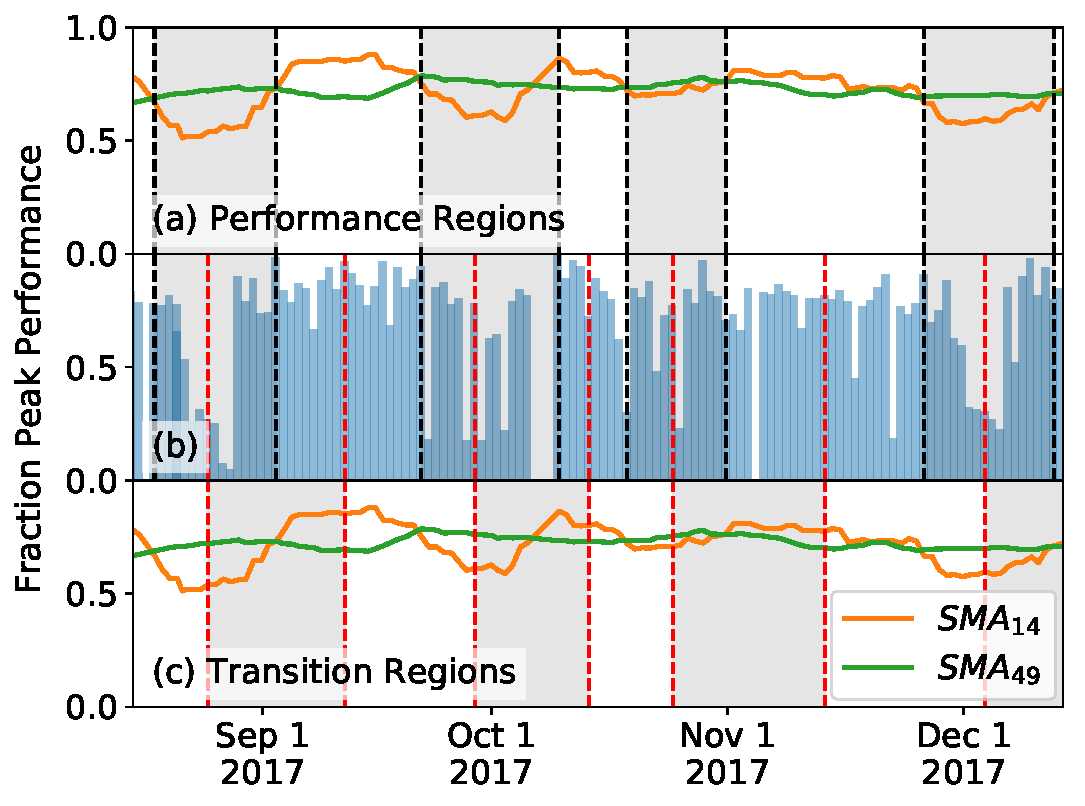
\includegraphics[width=1.0\columnwidth]{segment-explain}
    \vspace{-.35in}
    \caption{Example of overlaying two simple moving averages (SMAs) to identify (a) \emph{divergence regions} and (c) \emph{trend regions} in the Edison scratch2 IOR/fpp write dataset.  Middle pane (b) includes raw performance measurements (blue bars) with both SMA crossovers (black dashed lines) and divergence region centroids (red dashed lines).}
    \label{fig:segment-explain}
    % source: sc18_segments-explain.ipynb
\end{figure}

The data in Fig. \ref{fig:summary-heatmap} demonstrates that nominally optimal I/O performance for a given system evolves over time.
As a result, it is often not meaningful to express the performance of an application as being good or bad with respect to an absolute peak performance;
rather, "bad" performance (and its causes) should be classified with respect to what qualifies as "good" performance for a timescale of interest.
To address this issue, we propose applying simple moving averages (SMAs) as a means to identify correlated performance trends in production parallel file systems.
This approach has commonly been applied in the context of financial market technical analysis, where moving averages are used to attenuate the day-to-day volatility in the price movements of underlying assets and to help identify larger trends in these movements~\cite{james1968monthly,gunasekarage2001profitability}.

Given a time window of width $w$, we define the SMA for a metric $M$ at time $t$ as the average value of $M$ over ${-0.5w <= t < +0.5w}$;
when chosen to be sufficiently wide (e.g., $w = 49$ days), the resulting $\textup{SMA}_{49}$ provides a rapid visual means to identify performance degradation or recovery that lasts for $O(\textup{weeks})$.  Superimposing a second SMA with a shorter window, such as $\textup{SMA}_{14}$, then allows us to distinguish short-term performance anomalies that last for $O(\textup{days})$ from longer-term performance evolution.

In the following analysis, we apply this SMA-based approach to procedurally identify and classify performance variation at all time scales, ranging from long-term system health issues to transient performance loss due to probabilistic contention.
We define $\textup{SMA}_{short}$ and $\textup{SMA}_{long}$ as simple moving averages of widths $w_{short}$ and $w_{long}$, and for this study, chose $w_{short} = 14$ days and $w_{long} = 49$ days as a reasonable choice to focus on correlated performance events that occurred over $O(\textup{weeks})$.
That said, we found the exact choice of $w_{short}$ and $w_{long}$ to be somewhat arbitrary; adjusting these values by as much as $\pm 50\%$ did not affect the identification of the most significant events presented here.
In addition, a specific choice of $w$ does not preclude analyzing events longer or shorter than $w$, and we demonstrate methods to address this in Sections \ref{sec:results/longterm} and \ref{sec:results/shortterm}.

% J_{app, rw, sys}
We then partition a set of performance observations $J_{app, rw, sys}$ into \emph{divergence regions}, which are non-overlapping subsets of $J_{app, rw, sys}$ that are bounded by the crossover points between $\textup{SMA}_{long}$ and $\textup{SMA}_{short}$.
SMA crossover points are, again, a popular tool in technical analysis of financial markets, used to detect trend shifts in asset prices, often for predictive purposes\footnote{Though we note that the predictive capability of SMA crossovers is a source of controversy even in the financial community, and thus, we focus solely on using them as tools for managing volatility and detecting trends in historical datasets.} (e.g., as signals to buy or sell an asset based on the direction of the short and long-term SMAs at the time they crossover)~\cite{brock1992simple}.
Figure \ref{fig:segment-explain}a illustrates this partitioning of the IOR/fpp write workload measurements on Edison's scratch2 file system;
dashed lines represent the crossover points of $\textup{SMA}_{long}$ and $\textup{SMA}_{short}$, and divergence regions are shaded in alternating gray and white.
As Figure \ref{fig:segment-explain}a illustrates, using SMA crossovers to identify divergence regions results in temporally contiguous subsets of performance measurements that capture a period of time with consistently good (${\textup{SMA}_{short} > \textup{SMA}_{long}}$) or bad (${\textup{SMA}_{short} < \textup{SMA}_{long}}$) performance.

To understand the causes of the transitions between divergence regions, we also partition $J_{app, rw, sys}$ into \emph{trend regions}.
For each divergence region, we identify the temporally center-most observation as the centroid of that region, as illustrated in Figure \ref{fig:segment-explain}b, as red dashed lines.
We then define trend regions as those regions bounded by centroids (Figure \ref{fig:segment-explain}c), and each trend region overlaps with exactly two divergence regions and vice versa.
The principal difference between the two is that divergence regions contain observations that are uniformly good or uniformly bad, and trend regions capture performance transitioning from bad to good or vice versa.

